The consistency of the proposed ontologies and their compliance with ontology design best practices were verified using the HermiT reasoner integrated into Protégé\footnote{\url{http://protege.stanford.edu/}}~\cite{musen_protege_2015}, as well as the OOPS! tool\footnote{\url{https://oops.linkeddata.es/}}~\cite{poveda-villalon_oops_2014}.

\subsection{Population and validation of the address ontology}

The address ontology is also evaluated by populating it with three address datasets for Paris: two contemporary sources, OpenStreetMap (OSM) and the French National Address Database (BAN), and one historical source consisting of addresses extracted from the nineteenth-century Paris trade directories~\cite{abadie_benchmark_2022}. The integration process for these sources comprises three steps: (1) identifying the landmarks and spatial relationships composing the addresses, (2) structuring each address according to the proposed model, and (3) linking addresses referring to the same target.

\begin{table}[htbp]
    \centering
    \begin{tabular}{|l|l|l|l|l|l|l|}
    \hline
        num & rep & street\_name & postcode & city & lon & lat \\ \hline
        5 & & Boulevard Saint-Martin & 75003 & Paris 3rd & 2.361407 & 48.867933 \\
        134 & & Boulevard Raspail & 75006 & Paris 6th & 2.309998 & 48.86011 \\
        4 & & Rue Regnard & 75006 & Paris 6th & 2.338073 & 48.849885 \\
        48 & bis & Rue de Rivoli & 75004 & Paris 4th & 2.35448 & 48.85690 \\ \hline
    \end{tabular}
    \caption{Extract from a BAN file for the city of Paris. The address locations (provided by the \texttt{lat} and \texttt{lon} fields) in the BAN do not follow a single positioning rule. For each address, the method used to determine the location is specified (postal delivery point, entrance door, parcel centroid, etc.).}
    \label{tab:ban_sample}
\end{table}

The first step is straightforward for OSM and BAN data, which consist of postal addresses whose components are already separated. Structuring the historical addresses extracted from the Paris trade directories, which are more organic in nature (Figure~\ref{fig:exemple_modelisation_adresse}), is considerably more difficult, and off-the-shelf parsing tools such as LibPostal\footnote{\url{https://github.com/openvenues/libpostal}} fail to process them correctly. We therefore structured these addresses manually. The data from each source are then formatted as CSV or JSON, possibly after minor restructuring. For example, the BAN data (Table~\ref{tab:ban_sample}) are adapted by creating a \texttt{house\_number} field that concatenates the \texttt{num} and \texttt{rep} fields.

A mapping is defined for each source to specify how addresses should be converted into RDF according to the proposed ontology. This mapping identifies the landmarks and spatial relationships involved. We use Ontotext Refine\footnote{\url{https://www.ontotext.com/products/ontotext-refine/}} to construct these addresses. For a BAN file, the mapping creates nine resources: one \texttt{Address}, four \texttt{AddressSegment} resources, and four \texttt{Landmark} resources (\texttt{HouseNumber}, \texttt{Thoroughfare}, \texttt{PostalCode}, and \texttt{City}). The resulting graph contains duplicate landmark resources because addresses are created independently. For example, addresses located along the same street each generate a distinct resource describing that street. The final step therefore consists in removing duplicates using SPARQL queries: landmarks of the same type, having similar names and equivalent spatial relationships, are merged.

Once populated, we verified that the ontology can answer the predefined competency questions, translated into SPARQL queries. For example, the query retrieving all addresses targeting a place located along a given street (here, Rue du Dahomey) returns 16 addresses together with their coordinates, which are mapped in Figure~\ref{fig:localisation_adresses_rue_dahomey_paris}.

\begin{figure}[ht]
\begin{center}
 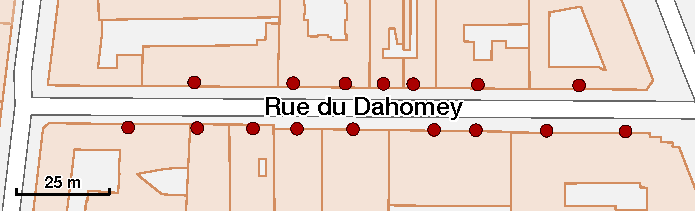
\includegraphics[width=0.85\textwidth]{images/localisation_adresses_rue_dahomey_paris.pdf}
 \caption{Location of addresses whose target is located along Rue du Dahomey.}
 \label{fig:localisation_adresses_rue_dahomey_paris}
\end{center}
\end{figure}

\subsection{Population and validation of the temporal evolution ontology}

To populate the ontology describing the temporal evolution of geographic landmarks, we used Wikidata data on the streets of Paris. These data include information such as creation dates and the successive official names of streets, together with their start and end dates of validity. From these data, we create \texttt{Thoroughfare} landmarks, name attributes together with their successive versions, and the corresponding changes.

Wikidata describes the successive states of streets. Therefore, for each state, we create two changes indicating respectively the beginning and the end of the state's validity. As a consequence, all changes are initially created independently and may therefore be duplicated. They must subsequently be merged using SPARQL queries.

Only a subset of the competency questions presented in Section~\ref{sect:prop_evolution_temporelle} could be translated into SPARQL queries, since this dataset is limited to the historical evolution of streets.

The history of a geographic entity can be reconstructed either by querying all the changes applied to the entity or by rebuilding its successive versions from the available changes, as illustrated in Figure~\ref{fig:evolution_place_nation}. Here, the states are inferred from the recorded events and may differ depending on which events are taken into account.

\begin{figure}
\begin{center}
 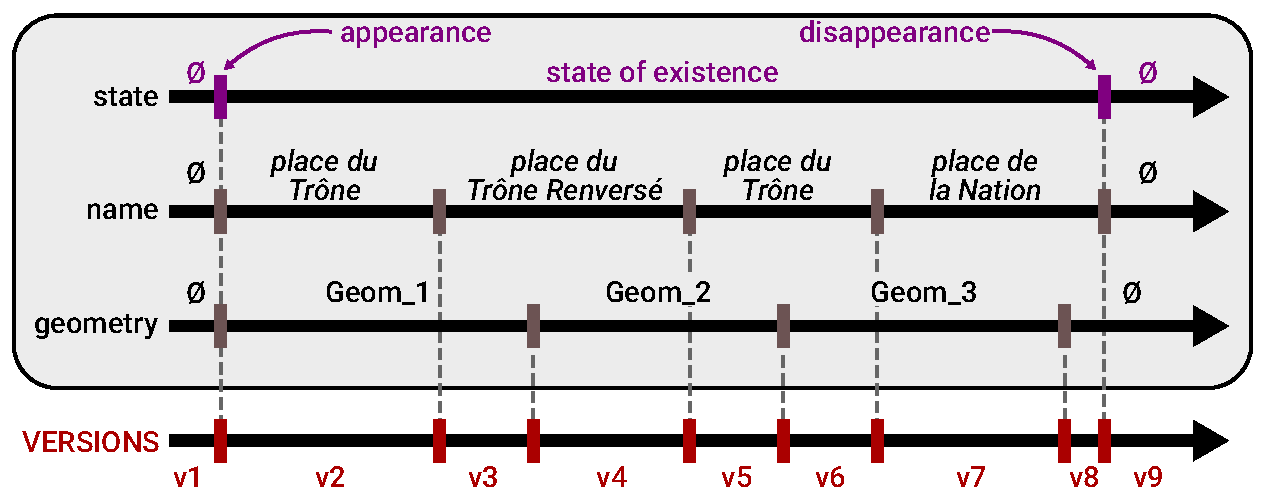
\includegraphics[width=\textwidth]{images/evolution_place_nation.pdf}
 \caption{Reconstruction of the successive states of Place de la Nation from the recorded changes.}
 \label{fig:evolution_place_nation}
\end{center}
\end{figure}